\chapter{Carbon: Cloud Workspaces}

\section{Purpose}


\section{Motivation}
\subsection{Reproducibility is crucial for science}
\subsection{Reproducibility is difficult for computational systems biology}
\subsection{Systems biology software is difficult to install}


\section{Solution}
\subsection{Framework for scientific web applications and personal workspaces}
\begin{figure}
  \centering
  \begin{subfigure}[b]{\textwidth}
    \includegraphics[width=\textwidth,page=9,trim=0.37cm 3.65cm 13.1cm 3.3cm, clip=true]{images/Figures.pdf}
    \caption{The Carbon landing page.}
    \label{Figure:carbon-login-landing}
  \end{subfigure}
  \begin{subfigure}[b]{\textwidth}
    \includegraphics[width=\textwidth,page=9,trim=13.1cm 3.65cm 0.37cm 3.3cm, clip=true]{images/Figures.pdf}
    \caption{Once the user is logged in, the navigation bar will populate with available applications.}
    \label{Figure:carbon-login-logged-in}
  \end{subfigure}
  \caption{Carbon provides a user-specific workspaces.}
  \label{Figure:carbon-login}
\end{figure}

\begin{figure}
  \centering
  \begin{subfigure}[b]{\textwidth}
    \includegraphics[width=\textwidth,page=10,trim=0.37cm 3.65cm 13.1cm 3.3cm, clip=true]{images/Figures.pdf}
    \caption{The left sidebar contains a collapsible directory tree view.
      Each directory also contains expandable option buttons for file creation, upload, and deletion.}
    \label{Figure:carbon-workspaces-view}
  \end{subfigure}
  \begin{subfigure}[b]{\textwidth}
    \includegraphics[width=\textwidth,page=10,trim=13.1cm 3.65cm 0.37cm 3.3cm, clip=true]{images/Figures.pdf}
    \caption{New folders can also be created anywhere within the directory tree.}
    \label{Figure:carbon-workspaces-new-folder}
  \end{subfigure}
  \caption{Workspace app is a plugin to Carbon that allows easy file management and browsing of model files.}
  \label{Figure:carbon-workspaces}
\end{figure}

\begin{figure}
  \centering
  \begin{subfigure}[b]{\textwidth}
    \includegraphics[width=\textwidth,page=11,trim=0.37cm 3.65cm 13.1cm 3.3cm, clip=true]{images/Figures.pdf}
    \caption{Users may create new files in the workspace by upload or copy and paste.}
    \label{Figure:carbon-workspaces-file-upload}
  \end{subfigure}
  \begin{subfigure}[b]{\textwidth}
    \includegraphics[width=\textwidth,page=11,trim=13.1cm 3.65cm 0.37cm 3.3cm, clip=true]{images/Figures.pdf}
    \caption{All files can be edited as text, but detected model files also uses Graphene to construct a network layout view.}
    \label{Figure:carbon-workspaces-model-view}
  \end{subfigure}
  \caption{}
  \label{Figure:carbon-workspaces-files}
\end{figure}

\begin{figure}
  \centering
  \begin{subfigure}[b]{\textwidth}
    \includegraphics[width=\textwidth,page=12,trim=0.37cm 3.65cm 13.1cm 3.3cm, clip=true]{images/Figures.pdf}
    \caption{}
    \label{Figure:}
  \end{subfigure}
  \begin{subfigure}[b]{\textwidth}
    \includegraphics[width=\textwidth,page=12,trim=13.1cm 3.65cm 0.37cm 3.3cm, clip=true]{images/Figures.pdf}
    \caption{}
    \label{Figure:}
  \end{subfigure}
  \caption{}
  \label{Figure:}
\end{figure}

\begin{figure}
  \centering
  \begin{subfigure}[b]{\textwidth}
    \includegraphics[width=\textwidth,page=13,trim=0.37cm 3.65cm 13.1cm 3.3cm, clip=true]{images/Figures.pdf}
    \caption{}
    \label{Figure:}
  \end{subfigure}
  \begin{subfigure}[b]{\textwidth}
    \includegraphics[width=\textwidth,page=13,trim=13.1cm 3.65cm 0.37cm 3.3cm, clip=true]{images/Figures.pdf}
    \caption{}
    \label{Figure:}
  \end{subfigure}
  \caption{}
  \label{Figure:}
\end{figure}

\begin{figure}
  \centering
  \includegraphics[width=\textwidth,page=14,trim=0.37cm .65cm 0.37cm 0.3cm, clip=true]{images/Figures.pdf}
  \caption{}
  \label{Figure:}
\end{figure}

\subsection{Python environment for model exploration, analysis, and curation}
\subsection{Convert standard model formats to IPython notebooks}


\section{Implementation}
\subsection{Server Architecture}
\subsubsection{Express.js and Flask}
\subsubsection{MongoDB}
\subsection{Workspace Isolation}
\subsubsection{Linux Containers}
\subsubsection{Services and Ports}
\subsection{Asynchronous Programming}
\subsubsection{Highly Nested Callbacks}
\subsubsection{Use of Promises}
\subsection{Conversion of model formats to IPython notebooks}

\section{Future Directions}
\subsection{Security}
